\documentclass[aspectratio=169, table]{beamer}

\usepackage{colortbl}
\usepackage{xcolor}
\usepackage{listings}
\usepackage{tikz}
\usepackage{pgfplots}
\usepgfplotslibrary{polar}
\usetikzlibrary{arrows.meta, positioning, calc}

\usetheme{Pradita}


\usepackage{listings}
\lstdefinestyle{SqlStyle}{
language=SQL,
basicstyle=\ttfamily\footnotesize,
morekeywords={REAL, TEXT, REFERENCES},
keywordstyle=\color{blue},
commentstyle=\color{gray},
stringstyle=\color{red},
breaklines=true,
showstringspaces=false,
tabsize=2,
captionpos=b,
numbers=left,
numberstyle=\tiny\color{gray},
frame=lines,
backgroundcolor=\color{lightgray!10},
comment=[l]{//},
morecomment=[s]{/*}{*/},
commentstyle=\color{gray}\ttfamily,
string=[s]{'}{'},
morestring=[s]{"}{"},
%	stringstyle=\color{teal}\ttfamily,
%	showstringspaces=false
}

\lstdefinelanguage{bash} {
keywords={},
basicstyle=\ttfamily\small,
keywordstyle=\color{blue}\bfseries,
ndkeywords={iex},
ndkeywordstyle=\color{purple}\bfseries,
sensitive=true,
commentstyle=\color{gray},
stringstyle=\color{red},
numbers=left,
numberstyle=\tiny\color{gray},
breaklines=true,
frame=lines,
backgroundcolor=\color{lightgray!10},
tabsize=2,
comment=[l]{\#},
morecomment=[s]{/*}{*/},
commentstyle=\color{gray}\ttfamily,
stringstyle=\color{purple}\ttfamily,
showstringspaces=false
}

% Define Java language style for listings
\lstdefinestyle{JavaScript}{
	language=Java,
	basicstyle=\ttfamily\footnotesize,
	keywordstyle=\color{blue},
	commentstyle=\color{gray},
	stringstyle=\color{red},
	breaklines=true,
	showstringspaces=false,
	tabsize=4,
	captionpos=b,
	numbers=left,
	numberstyle=\tiny\color{gray},
	frame=lines,
	backgroundcolor=\color{lightgray!10},
	comment=[l]{//},
	morecomment=[s]{/*}{*/},
	commentstyle=\color{gray}\ttfamily,
	string=[s]{'}{'},
	morestring=[s]{"}{"},
	%	stringstyle=\color{teal}\ttfamily,
	%	showstringspaces=false
}

\title{\Huge TDWI BI and AI \\
\vspace{10pt}
 Maturity Model}
\subtitle{IT140704 - Big Data for Business}
%\date[Serial]{Penggunaan Large Language Model untuk Pengajaran}
\author{\textbf{Alfa Yohannis}}
\begin{document}

\frame{\titlepage}


\begin{frame}[fragile]
\frametitle{Contents}
\vspace{20pt}
\begin{columns}[t]
	\column{0.5\textwidth}
	\tableofcontents[sections={1-5}]
	
	\column{0.5\textwidth}
	\tableofcontents[sections={6-20}]
\end{columns}
\end{frame}

\begin{frame}{\hfill}
	\centering
	\Huge{\textbf{How can an organization identify the current state of its Big Data initiative and determine how to improve it?}}
\end{frame}


\section{Value and Purpose of the Model}

\begin{frame}{Value and Purpose of the Model}
	\vspace{20pt}
	
	The TDWI Business Intelligence (BI) and Artificial Intelligence (AI) maturity model 
	serves as a framework to evaluate how effectively organizations leverage data, analytics, 
	and AI strategically. Its key purposes are:
	
	\begin{itemize}
		\item \textbf{Assess current state:} identify the organization’s position on the maturity spectrum.
		\item \textbf{Spot gaps:} reveal weaknesses in data infrastructure, governance, or skills.
		\item \textbf{Guide transformation:} provide phased improvement paths aligned with business strategy.
		\item \textbf{Maximize value:} ensure BI and AI investments drive efficiency, innovation, and growth.
	\end{itemize}
	
\end{frame}

\section{Introduction}

\begin{frame}{Introduction}
	\vspace{20pt}
	
	Rapid advances in \textit{Business Intelligence} (BI) and \textit{Artificial Intelligence} (AI) 
	are transforming how organizations leverage data for strategic decisions.  
	\begin{itemize}
		\item \textbf{BI} delivers insights through reporting, descriptive analytics, and visualization.  
		\item \textbf{AI} extends these with prediction, recommendation, and automation.  
		\item Integrated BI+AI boosts efficiency and fuels innovation, e.g., customer personalization, 
		anomaly detection, and Generative AI for knowledge work.  
		\item Yet adoption varies widely: some remain at basic reporting, while mature organizations 
		operate with integrated architectures, governance, and a data-driven culture.  
	\end{itemize}
	
\end{frame}

\section{Key Trends in BI and AI}

\begin{frame}{Key Trends in BI and AI}
	\vspace{20pt}
	
	Current BI and AI development highlights several transformative trends:  
	\begin{itemize}
		\item \textbf{Self-service analytics with GenAI:} natural language queries and automated insights.  
		\item \textbf{Data \& AI governance:} transparency, bias control, and regulatory compliance.  
		\item \textbf{Cloud \& Lakehouse integration:} scalable platforms unifying BI and AI needs.  
		\item \textbf{Emerging roles:} MLOps and AIOps for lifecycle and operational management.  
		\item \textbf{Data as product:} managing and monetizing data with product principles.  
	\end{itemize}
	
	These trends show that BI+AI evolution is not just technical but also cultural and strategic.
	
\end{frame}


\section{Model Dimensions}

\begin{frame}{Model Dimensions}
	\vspace{20pt}
	\centering
	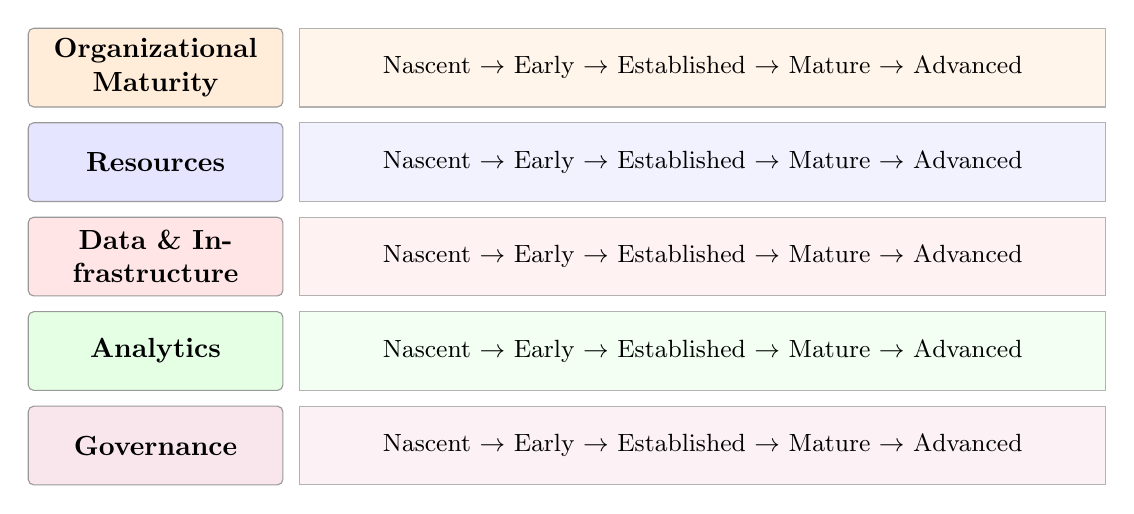
\begin{tikzpicture}[font=\small, node distance=1.2cm]
		\tikzset{
			dim/.style={draw=black!40, rounded corners=2pt, text width=3cm, minimum height=1cm, align=center, font=\bfseries},
			levels/.style={draw=black!30, text width=10cm, minimum height=1cm, align=center}
		}
		\node[dim, fill=orange!15] (d1) {Organizational Maturity};
		\node[dim, fill=blue!10, below of=d1] (d2) {Resources};
		\node[dim, fill=red!10, below of=d2] (d3) {Data \& Infrastructure};
		\node[dim, fill=green!10, below of=d3] (d4) {Analytics};
		\node[dim, fill=purple!10, below of=d4] (d5) {Governance};
		
		\node[levels, fill=orange!8, right=0.2cm of d1] {Nascent $\rightarrow$ Early $\rightarrow$ Established $\rightarrow$ Mature $\rightarrow$ Advanced};
		\node[levels, fill=blue!5, right=0.2cm of d2] {Nascent $\rightarrow$ Early $\rightarrow$ Established $\rightarrow$ Mature $\rightarrow$ Advanced};
		\node[levels, fill=red!5, right=0.2cm of d3] {Nascent $\rightarrow$ Early $\rightarrow$ Established $\rightarrow$ Mature $\rightarrow$ Advanced};
		\node[levels, fill=green!5, right=0.2cm of d4] {Nascent $\rightarrow$ Early $\rightarrow$ Established $\rightarrow$ Mature $\rightarrow$ Advanced};
		\node[levels, fill=purple!5, right=0.2cm of d5] {Nascent $\rightarrow$ Early $\rightarrow$ Established $\rightarrow$ Mature $\rightarrow$ Advanced};
	\end{tikzpicture}
\end{frame}

% Frame 1
\begin{frame}{Model Dimensions (1/2)}
	\vspace{20pt}
	
	The TDWI BI \& AI maturity model is built on five core dimensions that reflect 
	critical aspects of data and analytics management.  
	Each serves as a lens to evaluate strengths and weaknesses on the journey to becoming data-driven.
	
	\begin{itemize}
		\item \textbf{Organizational Maturity:} Covers strategy, leadership, culture, and resources. 
		Early stages often lack executive sponsorship and alignment, while mature organizations 
		foster strong leadership, cross-functional collaboration, and a pervasive data-driven culture.
		
		\item \textbf{Funding \& Talent:} Focuses on sustained investment, skills, and workforce readiness. 
		Mature organizations build structured programs for training, upskilling, and talent retention, 
		ensuring continuous innovation.
	\end{itemize}
	
\end{frame}

% Frame 2
\begin{frame}{Model Dimensions (2/2)}
	\vspace{20pt}
	
	\begin{itemize}
		\item \textbf{Data \& Infrastructure:} Examines data scope, platforms, architecture, and performance. 
		Early maturity shows siloed systems, while advanced levels adopt integrated, scalable, and secure 
		platforms such as warehouses, lakes, or lakehouses.
		
		\item \textbf{Analytics:} Reflects the breadth and depth of analytical capabilities, from basic 
		descriptive reports to predictive, prescriptive, and AI-driven insights. Mature organizations embed 
		analytics in operations and drive innovation through advanced AI and Generative AI.
		
		\item \textbf{Governance:} Includes data governance, AI governance, and supporting tools. 
		Covers compliance, risk management, stewardship, and ethical use, ensuring transparency, 
		trust, and accountability.
	\end{itemize}
	
	Understanding these five dimensions enables organizations to map their position 
	and set improvement priorities aligned with business context.
	
\end{frame}

\section{Maturity Stages}

% Frame 1
\begin{frame}{Maturity Stages (1/2)}
	\vspace{20pt}
	
	The TDWI BI \& AI maturity model describes five evolutionary stages.  
	Each stage reflects how organizations evolve in strategy, talent, data, analytics, and governance:
	
	\begin{enumerate}
		\item \textbf{Nascent:} Reliance on manual reporting and fragmented spreadsheets.  
		No formal strategy, limited governance, and minimal leadership awareness of BI/AI value.  
		
		\item \textbf{Early:} Basic dashboards or initial data warehouses appear.  
		Analytics remain descriptive and departmental, with integration challenges and skills gaps.  
		
		\item \textbf{Established:} Broader BI adoption across functions.  
		Data integration improves via ETL or pipelines, governance becomes more structured, 
		and early predictive or ML experiments begin.  
	\end{enumerate}
	
\end{frame}

% Frame 2
\begin{frame}{Maturity Stages (2/2)}
	\vspace{20pt}
	
	\begin{enumerate}
		\setcounter{enumi}{3} % continue numbering from 4
		\item \textbf{Mature:} Advanced analytics and AI are operationalized at scale.  
		MLOps practices support production AI, while governance ensures ethics, 
		security, and compliance. Data and AI drive enterprise-wide decision-making.  
		
		\item \textbf{Advanced / Visionary:} Organizations lead with Generative AI, 
		augmented analytics, and automation.  
		Data is monetized as a strategic asset, with BI/AI embedded in innovation 
		and business models, positioning them as industry leaders.  
	\end{enumerate}
	
	Maturity stages are evolutionary: strong foundations must be built before advancing.  
	Knowing the current stage enables organizations to design a clear and realistic roadmap.  
	
\end{frame}

\section{Dimension Overview }

% Frame 1
\begin{frame}{Dimension Overview (1/3)}
	\vspace{20pt}
	
	\textbf{Nascent}
	\begin{itemize}
		\item Data/Infra: fragmented spreadsheets, poor quality, no integration.
		\item Analytics/Tech: manual reporting only, no BI/AI.
		\item Governance: no governance, no standards or policies.
		\item Org/Culture: low literacy, intuition-based decisions.
		\item Strategy/Value: no BI/AI strategy, data not treated as asset.
	\end{itemize}
	
	\textbf{Early}
	\begin{itemize}
		\item Data/Infra: simple warehouse or reports, limited integration.
		\item Analytics/Tech: dashboards for descriptive use, ad-hoc analysis.
		\item Governance: basic policies, inconsistent application.
		\item Org/Culture: some BI adoption, culture not embedded.
		\item Strategy/Value: BI seen as IT project, not business strategy.
	\end{itemize}
	
\end{frame}

% Frame 2
\begin{frame}{Dimension Overview (2/3)}
	\vspace{20pt}
	
	\textbf{Established}
	\begin{itemize}
		\item Data/Infra: ETL + data marts, improving data quality.
		\item Analytics/Tech: basic predictive models (forecasting, segmentation).
		\item Governance: formal governance with stewards and security.
		\item Org/Culture: literacy programs, senior support visible.
		\item Strategy/Value: BI supports core business processes.
	\end{itemize}
	
	\textbf{Mature}
	\begin{itemize}
		\item Data/Infra: modern lakehouse with real-time integration.
		\item Analytics/Tech: AI operationalized using MLOps.
		\item Governance: covers AI ethics, compliance, regulations.
		\item Org/Culture: strong data-driven culture, leadership use.
		\item Strategy/Value: analytics tied to KPIs like retention, supply chain.
	\end{itemize}
	
\end{frame}

% Frame 3
\begin{frame}{Dimension Overview (3/3)}
	\vspace{20pt}
	
	\textbf{Advanced / Visionary}
	\begin{itemize}
		\item Data/Infra: pioneers advanced tech, e.g., digital twins, federated platforms.
		\item Analytics/Tech: generative AI, augmented analytics, automation standard.
		\item Governance: proactive, adaptive, industry-leading practices.
		\item Org/Culture: high literacy at all levels, roles like Chief AI Officer.
		\item Strategy/Value: data monetized as product, BI/AI expertise as edge.
	\end{itemize}
	
\end{frame}

\section{From Current State to Next Stage}

% Frame 1
\begin{frame}{From Current State to Next Stage (1/2)}
	\vspace{20pt}
	
	\textbf{Identifying Current Position}
	\begin{itemize}
		\item Conduct self-assessment across five dimensions: organizational maturity, resources, data \& infrastructure, analytics, and governance.
		\item Use structured surveys or workshops to locate the current maturity stage.
	\end{itemize}
	
	\textbf{Setting Improvement Priorities}
	\begin{itemize}
		\item Nascent $\rightarrow$ Early: consolidate fragmented data, standardize basic reporting.  
		\item Early $\rightarrow$ Established: expand predictive analytics, formalize governance with stewards.  
		\item Established $\rightarrow$ Mature: implement MLOps, scale literacy programs, embed data culture.  
		\item Mature $\rightarrow$ Advanced: pursue AI-driven innovation, monetize data as a strategic asset.  
	\end{itemize}
\end{frame}

% Frame 2
\begin{frame}{From Current State to Next Stage (2/2)}
	\vspace{20pt}
	
	\textbf{Key Success Factors}
	\begin{itemize}
		\item Strong executive sponsorship and organizational alignment.  
		\item Resources: sustained funding, skills development, and specialized roles.  
		\item Technology investment: scalable data platforms (lakehouse, cloud analytics), automation, and MLOps.  
		\item Governance: enforce standards, ethical AI practices, and regulatory compliance.  
	\end{itemize}
	
	\textbf{Measuring Impact}
	\begin{itemize}
		\item Track KPIs: BI/AI adoption rates, cost savings, prediction accuracy, revenue impact.  
		\item Apply continuous improvement to sustain progress and adapt to business needs.  
	\end{itemize}
	
	\textit{Maturity transitions are iterative—not strictly linear—balancing people, resources, technology, and governance.}
\end{frame}



% Frame 1
\begin{frame}{Evaluation and Interpretation }
	\vspace{20pt}
	
	\textbf{Purpose of Scoring}
	\begin{itemize}
		\item Identify maturity gaps across BI and AI dimensions.  
		\item Prioritize investments, resources, and initiatives.  
		\item Build a measurable roadmap for staged improvement.  
	\end{itemize}
	
	\textbf{Scoring Approach}
	\begin{itemize}
		\item Maturity levels:  
		\begin{itemize}
			\item 1 = Nascent  
			\item 2 = Early  
			\item 3 = Established  
			\item 4 = Mature  
			\item 5 = Advanced / Visionary  
		\end{itemize}
		\item Assessment typically conducted via structured surveys, interviews, or workshops.  
	\end{itemize}
\end{frame}

% Frame 2
\begin{frame}{Evaluation and Interpretation (2/2)}
	\vspace{20pt}
	
	\textbf{Scoring Dimensions}
	\begin{itemize}
		\item \textbf{Organizational Maturity:} from ad-hoc, intuition-driven (1) to fully embedded enterprise-wide leadership and culture (5).  
		\item \textbf{Resources:} from no dedicated funding or skills (1) to continuous reinvestment and world-class talent programs (5).  
		\item \textbf{Data \& Infrastructure:} from fragmented spreadsheets (1) to real-time, scalable, federated platforms (5).  
		\item \textbf{Analytics:} from manual reporting (1) to advanced AI, automation, and Generative AI (5).  
		\item \textbf{Governance:} from no policies or oversight (1) to proactive, adaptive, industry-leading governance (5).  
	\end{itemize}
	
	\textit{Dimension scores form a quantitative profile of organizational maturity, guiding targeted and prioritized improvements.}
\end{frame}

% Frame 1
\begin{frame}{Evaluating Scores (1/3)}
	\vspace{20pt}
	\textbf{Assessment Approach}
	\begin{itemize}
		\item TDWI BI \& AI Maturity Assessment has \textasciitilde50 questions across five dimensions.  
		\item Organizations can be at different maturity stages in each dimension.  
		\item Questions may be single or grouped, and weighted by importance.  
		\item Each dimension has a maximum score of 20 points.  
	\end{itemize}
	
	\textbf{Scoring Method}
	\begin{itemize}
		\item Each dimension is scored separately.  
		\item An overall score is also calculated.  
		\item Output: maturity score per dimension + total maturity score.  
	\end{itemize}
\end{frame}

% Frame 2
\begin{frame}{Evaluating Scores (2/3)}
	\vspace{20pt}
	\textbf{Interpretation of Scores}
	\begin{itemize}
		\item Scores map to maturity stages as follows:  
	\end{itemize}
	
	\begin{center}
		\begin{tabular}{|>{\columncolor{white}}c|>{\columncolor{white}}c|}
			\hline
			\textbf{Score Range} & \textbf{Stage} \\ \hline
			$<$ 5   & Nascent \\ \hline
			7--10   & Early \\ \hline
			11--14  & Established \\ \hline
			15--18  & Mature \\ \hline
			19--20  & Visionary \\ \hline
		\end{tabular}
	\end{center}
	
	\begin{itemize}
		\item Example: Score of 11 in Organizational Maturity = Established stage.  
		\item Scores vary by dimension—BI \& AI programs evolve unevenly.  
	\end{itemize}
\end{frame}

% Frame 3
\begin{frame}{Evaluating Scores (3/3)}
	\vspace{20pt}
	\textbf{Sample Results}
	
	\begin{center}
		\setlength{\arrayrulewidth}{0.3mm} % thin black border
		\arrayrulecolor{black} % border color
		\begin{tabular}{|l|c|c|}
			\hline
			\textbf{Dimension} & \textbf{Score} & \textbf{Stage} \\ \hline
			Organizational Maturity & 10 & Early \\ \hline
			Resources              & 7  & Early \\ \hline
			Data \& Infrastructure & 11 & Established \\ \hline
			Analytics              & 4  & Nascent \\ \hline
			Governance             & 7  & Early \\ \hline
		\end{tabular}
	\end{center}
	
	\begin{itemize}
		\item Total Score: 39.  
		\item Interpretation: More advanced in data infrastructure, weaker in analytics and resources.  
		\item Dimensions don’t mature uniformly—gaps highlight priority areas for investment.  
	\end{itemize}
\end{frame}


% Frame 1
\begin{frame}{Reading Results (1/3)}
	\vspace{20pt}
	\textbf{Purpose of Interpretation}
	\begin{itemize}
		\item Scores are not just numbers; they signal strategic implications.  
		\item They help organizations understand their BI/AI condition and growth trajectory.  
	\end{itemize}
	
	\textbf{Gap Analysis}
	\begin{itemize}
		\item Compare actual vs. target maturity levels for each dimension.  
		\item Example: Data \& Infrastructure at 2 (Early) vs. target 4 (Mature).  
		Roadmap: strengthen integration, improve data quality, adopt modern platforms.  
	\end{itemize}
\end{frame}

% Frame 2
\begin{frame}{Reading Results (2/3)}
	\vspace{20pt}
	\textbf{Maturity Profile}
	\begin{itemize}
		\item Combine dimension scores into a holistic maturity profile.  
		\item Visualization options:  
		\begin{itemize}
			\item Radar chart – shows strengths vs. weaknesses across dimensions.  
			\item Heatmap – highlights biggest maturity gaps for prioritization.  
			\item Benchmarking – compare scores against industry peers or competitors.  
		\end{itemize}
	\end{itemize}
	
	\textbf{Strategic Interpretation}
	\begin{itemize}
		\item High Analytics + Low Governance = rapid innovation, but high compliance risk.  
		\item High Organizational Maturity + Low Resources = strong vision, weak execution capability.  
	\end{itemize}
\end{frame}

% Frame 3
\begin{frame}{Reading Results (3/3)}
	\vspace{20pt}
	\textbf{Prioritization of Improvements}
	\begin{itemize}
		\item Use evaluation results to determine improvement priorities by dimension.  
		\item Example: Large gap in Organizational Maturity → invest in literacy, leadership alignment, and change management programs.  
		\item Example: Gap in Resources → allocate budget, expand skills training, create specialized roles (e.g., data steward, ML engineer).  
	\end{itemize}
	
	\textbf{Key Takeaway}
	\begin{itemize}
		\item Maturity scores serve not only as diagnosis.  
		\item They act as a compass, guiding sustainable BI/AI transformation across people, resources, technology, and governance.  
	\end{itemize}
\end{frame}


\section{Business Case Example}

% Frame 1
\begin{frame}{Business Case Example (1/4)}
	\vspace{20pt}
	\textbf{Context}
	\begin{itemize}
		\item Large retail company with physical stores and e-commerce.  
		\item Manages millions of customer transactions monthly.  
		\item Assessed BI \& AI maturity using the TDWI model.  
	\end{itemize}
	
	\textbf{Dimension Scores}
	\begin{itemize}
		\item Organizational Maturity: 3 (Established) – BI adoption growing, but culture uneven.  
		\item Resources: 2 (Early) – limited advanced skills, small data science budget.  
		\item Data \& Infrastructure: 3 (Established) – warehouse integrated, but not real-time.  
		\item Analytics: 2 (Early) – descriptive dashboards only, no predictive or ML ops.  
		\item Governance: 2 (Early) – basic policies, no AI ethics or regulatory frameworks.  
	\end{itemize}
\end{frame}

% Frame 2
\begin{frame}{Business Case Example (2/4)}
	\vspace{20pt}
	\textbf{Interpretation of Results}
	\begin{itemize}
		\item Strategy is clear at the organizational level (score 3), but weak analytics, resources, and governance (score 2).  
		\item Creates a \textit{strategic aspiration gap}: vision for data-driven growth exists, but execution capability lags.  
		\item Radar chart shows asymmetry with low points in analytics, resources, and governance.  
		\item Insight: prioritize near-term investments in weak dimensions to balance maturity.  
	\end{itemize}
\end{frame}

% Frame 3
\begin{frame}{Business Case Example (3/4)}
	\vspace{20pt}
	\textbf{Strategic Recommendations}
	\begin{itemize}
		\item Organizational Maturity (3): strengthen leadership sponsorship, expand literacy programs.  
		\item Resources (2): invest in training, create a data science team, expand budget for advanced analytics.  
		\item Data \& Infrastructure (3): migrate to a lakehouse for real-time analytics and scalability.  
		\item Analytics (2): introduce predictive modeling for demand forecasting and product recommendations.  
		\item Governance (2): establish a data governance unit, adopt global compliance standards (e.g., GDPR, CCPA).  
	\end{itemize}
\end{frame}

% Frame 4
\begin{frame}{Business Case Example (4/4)}
	\vspace{20pt}
	\textbf{Expected Business Impact}
	\begin{enumerate}
		\item Improve inventory prediction accuracy, reducing overstock and cutting storage cost by up to 15\%.  
		\item Reduce legal and reputational risks in international markets with stronger governance and compliance.  
		\item Accelerate operational decision-making across physical stores and digital channels.  
		\item Enhance customer personalization, driving revenue growth and loyalty.  
	\end{enumerate}
	
	\textit{Key Lesson: BI \& AI maturity assessment is not just diagnosis—it drives targeted interventions that deliver measurable business value.}
\end{frame}


\section{Summary}

\begin{frame}{Summary}
	\vspace{20pt}
	
	\begin{itemize}
		\item TDWI’s BI \& AI Maturity Model provides a structured framework to assess and guide digital transformation progress.  
		\item Five dimensions: Organizational Maturity, Resources, Data \& Infrastructure, Analytics, and Governance.  
		\item Scoring highlights strengths and gaps; interpretation enables gap analysis and prioritization of improvements.  
		\item The assessment is not a static diagnosis but a dynamic roadmap for continuous advancement.  
		\item Supports a gradual transition toward \textit{Advanced / Visionary}, where BI \& AI drive innovation, monetization, and lasting competitive advantage.  
	\end{itemize}
	
\end{frame}



\end{document}
